\documentclass{paper}
\usepackage{mathrsfs,amsmath, wasysym, geometry, pstricks, graphicx, type1cm, lettrine, float, fancyhdr}
\usepackage[super]{nth}
\geometry{a4paper}
\usepackage{algorithm}
\usepackage{amsmath}
\usepackage{algpseudocode}
\usepackage{graphicx}
\usepackage{microtype}
\usepackage{pdfpages}
\PassOptionsToPackage{hyphens}{url}\usepackage{hyperref}\usepackage{hyperref}

\newcommand{\HRule}{\rule{\linewidth}{0.5mm}}
\usepackage{listings}
\definecolor{mygreen}{rgb}{0,0.6,0}
\definecolor{mygray}{rgb}{0.8,0.8,0.8}
\definecolor{mymauve}{rgb}{0.58,0,0.82}

\pagestyle{fancy}
\lhead{Storm \emph{Proposal}}
\lfoot{QUT EESS}

\begin{document}
\newpage
\begin{titlepage}
\begin{center}

\textsc{\LARGE ENB440 RF Techniques and Modern Applications}\\[0.75cm]

\begin{figure}[H]
\centering

\includegraphics[width=0.2\textwidth]{IMG/QUT} \\[0.75cm]
\end{figure}

\textsc{\Large ENB440 - Filter Design}\\[0.5cm]

% Title
\HRule \\[0.4cm]
{ \huge \bfseries Design Milestone 1 \\[0.4cm] }

\HRule \\[1.5cm]



\begin{minipage}{0.4\textwidth}
\begin{flushleft} \large
Grant \textsc{Kennedy} \\
\emph{n8566712}\\
\end{flushleft}
\end{minipage}
\begin{minipage}{0.4\textwidth}
\begin{flushright} \large
Blake \textsc{Fuller} \\
\emph{n8598819}\\
\end{flushright}
\end{minipage}

\vfill

% Bottom of the page
{\large \today}
\end{center}
\end{titlepage}

\section{Executive Summary}


\newpage
\tableofcontents

\newpage
\section{Scope}


\newpage
\section{Line Impedance Calculations}
\subsection{Hand Calculations}
First we found the ABCD parameters for the circuit shown in Figure~\ref{fig:theoretical_circuit}. Once found they were converted to scattering parameters.

\begin{figure}[H]
	\centering
	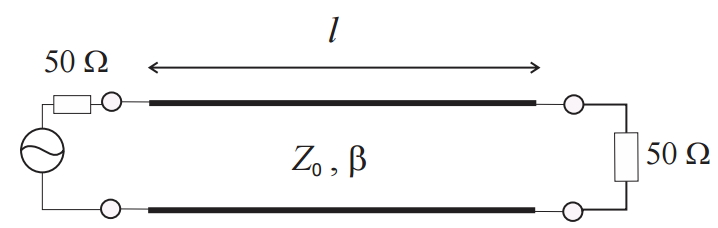
\includegraphics[scale=0.5]{IMG/theoretical_circuit}
	\caption{Theoretical stripline circuit}
	\label{fig:theoretical_circuit}
\end{figure}

This circuit consists of two 50$\Omega$ loads and two sections of transmission line with an electrical length of $\lambda$ and an impedence($Z_0$) of $70\Omega$. The wave number ($\beta$) is given by:
$$\beta = \frac{2\pi}{\lambda}$$
The unsimplified ABCD representation for this circuit is the following:
$$\begin{bmatrix}
A & B\\
C & D
\end{bmatrix} = 
\begin{bmatrix}
1 & 50\\
0 & 1
\end{bmatrix}
\begin{bmatrix}
cos(\beta\l) & j70sin(\beta\l)\\
\frac{jsin(\beta\l)}{70} & cos(\beta\l)
\end{bmatrix}
\begin{bmatrix}
1 & 50\\
0 & 1
\end{bmatrix}
\begin{bmatrix}
cos(\beta\l) & j70sin(\beta\l)\\
\frac{jsin(\beta\l)}{70} & cos(\beta\l)
\end{bmatrix}
$$
As $\beta\l=2\pi$ the sin terms are 0 and the cos terms become 1. The results for the ABCD matrix are as follows:
$$\begin{bmatrix}
A & B\\
C & D
\end{bmatrix} = 
\begin{bmatrix}
1 & 100\\
0 & 1
\end{bmatrix}
$$
The conversion from ABCD to scattering parameters is shown here:
\begin{align}
S_{11} &=\frac{A+B/Z_0-CZ_0-D}{A+B/Z_0+CZ_0+D}\\
S_{11} &=\frac{1+100/70-0-1}{1+100/70+0+1}\\
S_{11} &=\frac{5}{12}\\
&= 20log(S_{11})= -7.6042dB
\end{align}
\begin{align}
S_{12} &= \frac{2(AD-BC)}{A+B/Z_0+CZ_0+D}\\
S_{12} &= \frac{2(1-0)}{1+100/70+0+1}\\
S_{12} &= \frac{7}{12} \\ 
&= 20log(S_{12})= -4.6817dB
\end{align}
\begin{align}
S_{21} &= \frac{2}{A+B/Z_0+CZ_0+D}\\
S_{21} &= \frac{2}{1+100/70+0+1}\\
S_{21} &= \frac{7}{12} \\
&= 20log(S_{21})= -4.6817dB
\end{align}
\begin{align}
S_{22} &= \frac{-A+B/Z_0-CZ_0+D}{A+B/Z_0 +CZ_0+D}\\
S_{22} &= \frac{-1+100/70-0+1}{1+100/70+0+1}\\
S_{22} &= \frac{5}{12} \\
&= 20log(S_{22})= -7.6042dB
\end{align}
\subsection{Computer Generated Results}
The National Instruments (NI) program TX-Line was used to generate an approximation of the microstrip geometry. The given laminate, impedance, frequency and electrical length information were input and the program output the microstrip width and length. \\

These values can be seen in the TX-Line GUI screenshop in figure ~\ref{fig:txline}  

\begin{figure}[H]
	\centering
	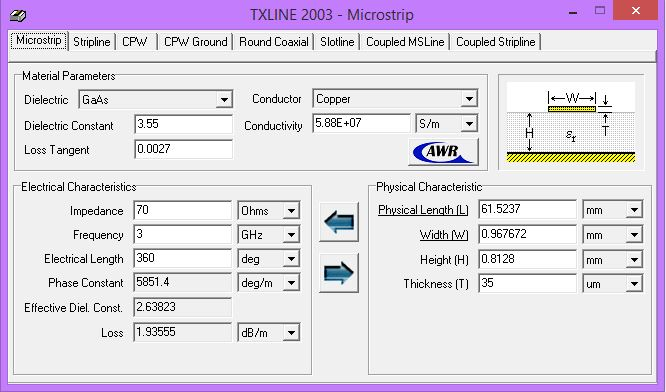
\includegraphics[scale=0.5]{IMG/txline}
	\caption{Screenshot of TX-Line program}
	\label{fig:txline}
\end{figure}

The following data was found from the results:

\begin{center}
	\begin{tabular}{c|c}
		\hline
		Characteristic & Result\\\hline\hline
		Phase Constant & 0.102126 rad/mm\\\hline
		Physical Length & 61.5237 mm\\	\hline
		Width & 0.967672 mm\\\hline
		Eff. Diel. Const. & 2.63823\\\hline
	\end{tabular}
\end{center}

\section{Modeling}
The stripline was modeled in CST, with a frequency range of 2GHz to 4GHz and port information at 3GHz.


\end{document}